\documentclass{article} % For LaTex2e
\usepackage{iclr2022_conference,times}
% Optional math commands from https://github.com/goodfeli/dlbook_notation.
%%%%% NEW MATH DEFINITIONS %%%%%

\usepackage{amsmath,amsfonts,bm}

% Mark sections of captions for referring to divisions of figures
\newcommand{\figleft}{{\em (Left)}}
\newcommand{\figcenter}{{\em (Center)}}
\newcommand{\figright}{{\em (Right)}}
\newcommand{\figtop}{{\em (Top)}}
\newcommand{\figbottom}{{\em (Bottom)}}
\newcommand{\captiona}{{\em (a)}}
\newcommand{\captionb}{{\em (b)}}
\newcommand{\captionc}{{\em (c)}}
\newcommand{\captiond}{{\em (d)}}

% Highlight a newly defined term
\newcommand{\newterm}[1]{{\bf #1}}


% Figure reference, lower-case.
\def\figref#1{figure~\ref{#1}}
% Figure reference, capital. For start of sentence
\def\Figref#1{Figure~\ref{#1}}
\def\twofigref#1#2{figures \ref{#1} and \ref{#2}}
\def\quadfigref#1#2#3#4{figures \ref{#1}, \ref{#2}, \ref{#3} and \ref{#4}}
% Section reference, lower-case.
\def\secref#1{section~\ref{#1}}
% Section reference, capital.
\def\Secref#1{Section~\ref{#1}}
% Reference to two sections.
\def\twosecrefs#1#2{sections \ref{#1} and \ref{#2}}
% Reference to three sections.
\def\secrefs#1#2#3{sections \ref{#1}, \ref{#2} and \ref{#3}}
% Reference to an equation, lower-case.
\def\eqref#1{equation~\ref{#1}}
% Reference to an equation, upper case
\def\Eqref#1{Equation~\ref{#1}}
% A raw reference to an equation---avoid using if possible
\def\plaineqref#1{\ref{#1}}
% Reference to a chapter, lower-case.
\def\chapref#1{chapter~\ref{#1}}
% Reference to an equation, upper case.
\def\Chapref#1{Chapter~\ref{#1}}
% Reference to a range of chapters
\def\rangechapref#1#2{chapters\ref{#1}--\ref{#2}}
% Reference to an algorithm, lower-case.
\def\algref#1{algorithm~\ref{#1}}
% Reference to an algorithm, upper case.
\def\Algref#1{Algorithm~\ref{#1}}
\def\twoalgref#1#2{algorithms \ref{#1} and \ref{#2}}
\def\Twoalgref#1#2{Algorithms \ref{#1} and \ref{#2}}
% Reference to a part, lower case
\def\partref#1{part~\ref{#1}}
% Reference to a part, upper case
\def\Partref#1{Part~\ref{#1}}
\def\twopartref#1#2{parts \ref{#1} and \ref{#2}}

\def\ceil#1{\lceil #1 \rceil}
\def\floor#1{\lfloor #1 \rfloor}
\def\1{\bm{1}}
\newcommand{\train}{\mathcal{D}}
\newcommand{\valid}{\mathcal{D_{\mathrm{valid}}}}
\newcommand{\test}{\mathcal{D_{\mathrm{test}}}}

\def\eps{{\epsilon}}


% Random variables
\def\reta{{\textnormal{$\eta$}}}
\def\ra{{\textnormal{a}}}
\def\rb{{\textnormal{b}}}
\def\rc{{\textnormal{c}}}
\def\rd{{\textnormal{d}}}
\def\re{{\textnormal{e}}}
\def\rf{{\textnormal{f}}}
\def\rg{{\textnormal{g}}}
\def\rh{{\textnormal{h}}}
\def\ri{{\textnormal{i}}}
\def\rj{{\textnormal{j}}}
\def\rk{{\textnormal{k}}}
\def\rl{{\textnormal{l}}}
% rm is already a command, just don't name any random variables m
\def\rn{{\textnormal{n}}}
\def\ro{{\textnormal{o}}}
\def\rp{{\textnormal{p}}}
\def\rq{{\textnormal{q}}}
\def\rr{{\textnormal{r}}}
\def\rs{{\textnormal{s}}}
\def\rt{{\textnormal{t}}}
\def\ru{{\textnormal{u}}}
\def\rv{{\textnormal{v}}}
\def\rw{{\textnormal{w}}}
\def\rx{{\textnormal{x}}}
\def\ry{{\textnormal{y}}}
\def\rz{{\textnormal{z}}}

% Random vectors
\def\rvepsilon{{\mathbf{\epsilon}}}
\def\rvtheta{{\mathbf{\theta}}}
\def\rva{{\mathbf{a}}}
\def\rvb{{\mathbf{b}}}
\def\rvc{{\mathbf{c}}}
\def\rvd{{\mathbf{d}}}
\def\rve{{\mathbf{e}}}
\def\rvf{{\mathbf{f}}}
\def\rvg{{\mathbf{g}}}
\def\rvh{{\mathbf{h}}}
\def\rvu{{\mathbf{i}}}
\def\rvj{{\mathbf{j}}}
\def\rvk{{\mathbf{k}}}
\def\rvl{{\mathbf{l}}}
\def\rvm{{\mathbf{m}}}
\def\rvn{{\mathbf{n}}}
\def\rvo{{\mathbf{o}}}
\def\rvp{{\mathbf{p}}}
\def\rvq{{\mathbf{q}}}
\def\rvr{{\mathbf{r}}}
\def\rvs{{\mathbf{s}}}
\def\rvt{{\mathbf{t}}}
\def\rvu{{\mathbf{u}}}
\def\rvv{{\mathbf{v}}}
\def\rvw{{\mathbf{w}}}
\def\rvx{{\mathbf{x}}}
\def\rvy{{\mathbf{y}}}
\def\rvz{{\mathbf{z}}}

% Elements of random vectors
\def\erva{{\textnormal{a}}}
\def\ervb{{\textnormal{b}}}
\def\ervc{{\textnormal{c}}}
\def\ervd{{\textnormal{d}}}
\def\erve{{\textnormal{e}}}
\def\ervf{{\textnormal{f}}}
\def\ervg{{\textnormal{g}}}
\def\ervh{{\textnormal{h}}}
\def\ervi{{\textnormal{i}}}
\def\ervj{{\textnormal{j}}}
\def\ervk{{\textnormal{k}}}
\def\ervl{{\textnormal{l}}}
\def\ervm{{\textnormal{m}}}
\def\ervn{{\textnormal{n}}}
\def\ervo{{\textnormal{o}}}
\def\ervp{{\textnormal{p}}}
\def\ervq{{\textnormal{q}}}
\def\ervr{{\textnormal{r}}}
\def\ervs{{\textnormal{s}}}
\def\ervt{{\textnormal{t}}}
\def\ervu{{\textnormal{u}}}
\def\ervv{{\textnormal{v}}}
\def\ervw{{\textnormal{w}}}
\def\ervx{{\textnormal{x}}}
\def\ervy{{\textnormal{y}}}
\def\ervz{{\textnormal{z}}}

% Random matrices
\def\rmA{{\mathbf{A}}}
\def\rmB{{\mathbf{B}}}
\def\rmC{{\mathbf{C}}}
\def\rmD{{\mathbf{D}}}
\def\rmE{{\mathbf{E}}}
\def\rmF{{\mathbf{F}}}
\def\rmG{{\mathbf{G}}}
\def\rmH{{\mathbf{H}}}
\def\rmI{{\mathbf{I}}}
\def\rmJ{{\mathbf{J}}}
\def\rmK{{\mathbf{K}}}
\def\rmL{{\mathbf{L}}}
\def\rmM{{\mathbf{M}}}
\def\rmN{{\mathbf{N}}}
\def\rmO{{\mathbf{O}}}
\def\rmP{{\mathbf{P}}}
\def\rmQ{{\mathbf{Q}}}
\def\rmR{{\mathbf{R}}}
\def\rmS{{\mathbf{S}}}
\def\rmT{{\mathbf{T}}}
\def\rmU{{\mathbf{U}}}
\def\rmV{{\mathbf{V}}}
\def\rmW{{\mathbf{W}}}
\def\rmX{{\mathbf{X}}}
\def\rmY{{\mathbf{Y}}}
\def\rmZ{{\mathbf{Z}}}

% Elements of random matrices
\def\ermA{{\textnormal{A}}}
\def\ermB{{\textnormal{B}}}
\def\ermC{{\textnormal{C}}}
\def\ermD{{\textnormal{D}}}
\def\ermE{{\textnormal{E}}}
\def\ermF{{\textnormal{F}}}
\def\ermG{{\textnormal{G}}}
\def\ermH{{\textnormal{H}}}
\def\ermI{{\textnormal{I}}}
\def\ermJ{{\textnormal{J}}}
\def\ermK{{\textnormal{K}}}
\def\ermL{{\textnormal{L}}}
\def\ermM{{\textnormal{M}}}
\def\ermN{{\textnormal{N}}}
\def\ermO{{\textnormal{O}}}
\def\ermP{{\textnormal{P}}}
\def\ermQ{{\textnormal{Q}}}
\def\ermR{{\textnormal{R}}}
\def\ermS{{\textnormal{S}}}
\def\ermT{{\textnormal{T}}}
\def\ermU{{\textnormal{U}}}
\def\ermV{{\textnormal{V}}}
\def\ermW{{\textnormal{W}}}
\def\ermX{{\textnormal{X}}}
\def\ermY{{\textnormal{Y}}}
\def\ermZ{{\textnormal{Z}}}

% Vectors
\def\vzero{{\bm{0}}}
\def\vone{{\bm{1}}}
\def\vmu{{\bm{\mu}}}
\def\vtheta{{\bm{\theta}}}
\def\va{{\bm{a}}}
\def\vb{{\bm{b}}}
\def\vc{{\bm{c}}}
\def\vd{{\bm{d}}}
\def\ve{{\bm{e}}}
\def\vf{{\bm{f}}}
\def\vg{{\bm{g}}}
\def\vh{{\bm{h}}}
\def\vi{{\bm{i}}}
\def\vj{{\bm{j}}}
\def\vk{{\bm{k}}}
\def\vl{{\bm{l}}}
\def\vm{{\bm{m}}}
\def\vn{{\bm{n}}}
\def\vo{{\bm{o}}}
\def\vp{{\bm{p}}}
\def\vq{{\bm{q}}}
\def\vr{{\bm{r}}}
\def\vs{{\bm{s}}}
\def\vt{{\bm{t}}}
\def\vu{{\bm{u}}}
\def\vv{{\bm{v}}}
\def\vw{{\bm{w}}}
\def\vx{{\bm{x}}}
\def\vy{{\bm{y}}}
\def\vz{{\bm{z}}}

% Elements of vectors
\def\evalpha{{\alpha}}
\def\evbeta{{\beta}}
\def\evepsilon{{\epsilon}}
\def\evlambda{{\lambda}}
\def\evomega{{\omega}}
\def\evmu{{\mu}}
\def\evpsi{{\psi}}
\def\evsigma{{\sigma}}
\def\evtheta{{\theta}}
\def\eva{{a}}
\def\evb{{b}}
\def\evc{{c}}
\def\evd{{d}}
\def\eve{{e}}
\def\evf{{f}}
\def\evg{{g}}
\def\evh{{h}}
\def\evi{{i}}
\def\evj{{j}}
\def\evk{{k}}
\def\evl{{l}}
\def\evm{{m}}
\def\evn{{n}}
\def\evo{{o}}
\def\evp{{p}}
\def\evq{{q}}
\def\evr{{r}}
\def\evs{{s}}
\def\evt{{t}}
\def\evu{{u}}
\def\evv{{v}}
\def\evw{{w}}
\def\evx{{x}}
\def\evy{{y}}
\def\evz{{z}}

% Matrix
\def\mA{{\bm{A}}}
\def\mB{{\bm{B}}}
\def\mC{{\bm{C}}}
\def\mD{{\bm{D}}}
\def\mE{{\bm{E}}}
\def\mF{{\bm{F}}}
\def\mG{{\bm{G}}}
\def\mH{{\bm{H}}}
\def\mI{{\bm{I}}}
\def\mJ{{\bm{J}}}
\def\mK{{\bm{K}}}
\def\mL{{\bm{L}}}
\def\mM{{\bm{M}}}
\def\mN{{\bm{N}}}
\def\mO{{\bm{O}}}
\def\mP{{\bm{P}}}
\def\mQ{{\bm{Q}}}
\def\mR{{\bm{R}}}
\def\mS{{\bm{S}}}
\def\mT{{\bm{T}}}
\def\mU{{\bm{U}}}
\def\mV{{\bm{V}}}
\def\mW{{\bm{W}}}
\def\mX{{\bm{X}}}
\def\mY{{\bm{Y}}}
\def\mZ{{\bm{Z}}}
\def\mBeta{{\bm{\beta}}}
\def\mPhi{{\bm{\Phi}}}
\def\mLambda{{\bm{\Lambda}}}
\def\mSigma{{\bm{\Sigma}}}

% Tensor
\DeclareMathAlphabet{\mathsfit}{\encodingdefault}{\sfdefault}{m}{sl}
\SetMathAlphabet{\mathsfit}{bold}{\encodingdefault}{\sfdefault}{bx}{n}
\newcommand{\tens}[1]{\bm{\mathsfit{#1}}}
\def\tA{{\tens{A}}}
\def\tB{{\tens{B}}}
\def\tC{{\tens{C}}}
\def\tD{{\tens{D}}}
\def\tE{{\tens{E}}}
\def\tF{{\tens{F}}}
\def\tG{{\tens{G}}}
\def\tH{{\tens{H}}}
\def\tI{{\tens{I}}}
\def\tJ{{\tens{J}}}
\def\tK{{\tens{K}}}
\def\tL{{\tens{L}}}
\def\tM{{\tens{M}}}
\def\tN{{\tens{N}}}
\def\tO{{\tens{O}}}
\def\tP{{\tens{P}}}
\def\tQ{{\tens{Q}}}
\def\tR{{\tens{R}}}
\def\tS{{\tens{S}}}
\def\tT{{\tens{T}}}
\def\tU{{\tens{U}}}
\def\tV{{\tens{V}}}
\def\tW{{\tens{W}}}
\def\tX{{\tens{X}}}
\def\tY{{\tens{Y}}}
\def\tZ{{\tens{Z}}}


% Graph
\def\gA{{\mathcal{A}}}
\def\gB{{\mathcal{B}}}
\def\gC{{\mathcal{C}}}
\def\gD{{\mathcal{D}}}
\def\gE{{\mathcal{E}}}
\def\gF{{\mathcal{F}}}
\def\gG{{\mathcal{G}}}
\def\gH{{\mathcal{H}}}
\def\gI{{\mathcal{I}}}
\def\gJ{{\mathcal{J}}}
\def\gK{{\mathcal{K}}}
\def\gL{{\mathcal{L}}}
\def\gM{{\mathcal{M}}}
\def\gN{{\mathcal{N}}}
\def\gO{{\mathcal{O}}}
\def\gP{{\mathcal{P}}}
\def\gQ{{\mathcal{Q}}}
\def\gR{{\mathcal{R}}}
\def\gS{{\mathcal{S}}}
\def\gT{{\mathcal{T}}}
\def\gU{{\mathcal{U}}}
\def\gV{{\mathcal{V}}}
\def\gW{{\mathcal{W}}}
\def\gX{{\mathcal{X}}}
\def\gY{{\mathcal{Y}}}
\def\gZ{{\mathcal{Z}}}

% Sets
\def\sA{{\mathbb{A}}}
\def\sB{{\mathbb{B}}}
\def\sC{{\mathbb{C}}}
\def\sD{{\mathbb{D}}}
% Don't use a set called E, because this would be the same as our symbol
% for expectation.
\def\sF{{\mathbb{F}}}
\def\sG{{\mathbb{G}}}
\def\sH{{\mathbb{H}}}
\def\sI{{\mathbb{I}}}
\def\sJ{{\mathbb{J}}}
\def\sK{{\mathbb{K}}}
\def\sL{{\mathbb{L}}}
\def\sM{{\mathbb{M}}}
\def\sN{{\mathbb{N}}}
\def\sO{{\mathbb{O}}}
\def\sP{{\mathbb{P}}}
\def\sQ{{\mathbb{Q}}}
\def\sR{{\mathbb{R}}}
\def\sS{{\mathbb{S}}}
\def\sT{{\mathbb{T}}}
\def\sU{{\mathbb{U}}}
\def\sV{{\mathbb{V}}}
\def\sW{{\mathbb{W}}}
\def\sX{{\mathbb{X}}}
\def\sY{{\mathbb{Y}}}
\def\sZ{{\mathbb{Z}}}

% Entries of a matrix
\def\emLambda{{\Lambda}}
\def\emA{{A}}
\def\emB{{B}}
\def\emC{{C}}
\def\emD{{D}}
\def\emE{{E}}
\def\emF{{F}}
\def\emG{{G}}
\def\emH{{H}}
\def\emI{{I}}
\def\emJ{{J}}
\def\emK{{K}}
\def\emL{{L}}
\def\emM{{M}}
\def\emN{{N}}
\def\emO{{O}}
\def\emP{{P}}
\def\emQ{{Q}}
\def\emR{{R}}
\def\emS{{S}}
\def\emT{{T}}
\def\emU{{U}}
\def\emV{{V}}
\def\emW{{W}}
\def\emX{{X}}
\def\emY{{Y}}
\def\emZ{{Z}}
\def\emSigma{{\Sigma}}

% entries of a tensor
% Same font as tensor, without \bm wrapper
\newcommand{\etens}[1]{\mathsfit{#1}}
\def\etLambda{{\etens{\Lambda}}}
\def\etA{{\etens{A}}}
\def\etB{{\etens{B}}}
\def\etC{{\etens{C}}}
\def\etD{{\etens{D}}}
\def\etE{{\etens{E}}}
\def\etF{{\etens{F}}}
\def\etG{{\etens{G}}}
\def\etH{{\etens{H}}}
\def\etI{{\etens{I}}}
\def\etJ{{\etens{J}}}
\def\etK{{\etens{K}}}
\def\etL{{\etens{L}}}
\def\etM{{\etens{M}}}
\def\etN{{\etens{N}}}
\def\etO{{\etens{O}}}
\def\etP{{\etens{P}}}
\def\etQ{{\etens{Q}}}
\def\etR{{\etens{R}}}
\def\etS{{\etens{S}}}
\def\etT{{\etens{T}}}
\def\etU{{\etens{U}}}
\def\etV{{\etens{V}}}
\def\etW{{\etens{W}}}
\def\etX{{\etens{X}}}
\def\etY{{\etens{Y}}}
\def\etZ{{\etens{Z}}}

% The true underlying data generating distribution
\newcommand{\pdata}{p_{\rm{data}}}
% The empirical distribution defined by the training set
\newcommand{\ptrain}{\hat{p}_{\rm{data}}}
\newcommand{\Ptrain}{\hat{P}_{\rm{data}}}
% The model distribution
\newcommand{\pmodel}{p_{\rm{model}}}
\newcommand{\Pmodel}{P_{\rm{model}}}
\newcommand{\ptildemodel}{\tilde{p}_{\rm{model}}}
% Stochastic autoencoder distributions
\newcommand{\pencode}{p_{\rm{encoder}}}
\newcommand{\pdecode}{p_{\rm{decoder}}}
\newcommand{\precons}{p_{\rm{reconstruct}}}

\newcommand{\laplace}{\mathrm{Laplace}} % Laplace distribution

\newcommand{\E}{\mathbb{E}}
\newcommand{\Ls}{\mathcal{L}}
\newcommand{\R}{\mathbb{R}}
\newcommand{\emp}{\tilde{p}}
\newcommand{\lr}{\alpha}
\newcommand{\reg}{\lambda}
\newcommand{\rect}{\mathrm{rectifier}}
\newcommand{\softmax}{\mathrm{softmax}}
\newcommand{\sigmoid}{\sigma}
\newcommand{\softplus}{\zeta}
\newcommand{\KL}{D_{\mathrm{KL}}}
\newcommand{\Var}{\mathrm{Var}}
\newcommand{\standarderror}{\mathrm{SE}}
\newcommand{\Cov}{\mathrm{Cov}}
% Wolfram Mathworld says $L^2$ is for function spaces and $\ell^2$ is for vectors
% But then they seem to use $L^2$ for vectors throughout the site, and so does
% wikipedia.
\newcommand{\normlzero}{L^0}
\newcommand{\normlone}{L^1}
\newcommand{\normltwo}{L^2}
\newcommand{\normlp}{L^p}
\newcommand{\normmax}{L^\infty}

\newcommand{\parents}{Pa} % See usage in notation.tex. Chosen to match Daphne's book.

\DeclareMathOperator*{\argmax}{arg\,max}
\DeclareMathOperator*{\argmin}{arg\,min}

\DeclareMathOperator{\sign}{sign}
\DeclareMathOperator{\Tr}{Tr}
\let\ab\allowbreak


%######## PHY293: Uncomment your submission name
\newcommand{\phyname}{}
%\newcommand{\phyname}{Progress Report}
%\newcommand{\phyname}{Final Report}

%######## PHY293: Put your Group Number here
%\newcommand{\gpnumber}{40}

\usepackage{hyperref}
\usepackage{xcolor}
\usepackage[normalem]{ulem}
\usepackage{url}
\usepackage{graphicx}
\usepackage{placeins}
\usepackage{float}
\usepackage{tikz}
\usepackage{multicol}
\usepackage{makecell}
\usepackage{amsmath}
\usepackage[table]{xcolor}

%######## PHY293: Put your project Title here
\title{The Output Resistance of a Power Supply: \\
An Introductory Resistance Exercise}

%######## PHY293: Put your names, student IDs and Emails here
\author{Karys Littlejohns\\
Student\# \\
karys.littlejohns@mail.utoronto.ca
\And
Peter Leong \\
Student\# 1010892955 \\
peter.leong@mail.utoronto.ca \\
\AND
}

% The \author macro works with any number of authors. There are two commands
% used to separate the names and addresses of multiple authors: \And and \AND.
%
% Using \And between authors leaves it to \LaTex{} to determine where to break
% the lines. Using \AND forces a linebreak at that point. So, if \LaTex{}
% puts 3 of 4 authors names on the first line, and the last on the second
% line, try using \AND instead of \And before the third author name.

\newcommand{\fix}{\marginpar{FIx}}
\newcommand{\new}{\marginpar{NEW}}

\iclrfinalcopy 
%######## PHY293: Document starts here
\begin{document}

\maketitle

\vspace{-6ex}

% \begin{abstract}

% ----Total Pages: \pageref{last_page}
% \end{abstract}

%\vspace{2ex}

\section{Introduction}

Sources of electricity produce a voltage potential across their terminals called an electromotive force (\textit{emf}) or an open circuit voltage, $V_{\infty}$.
In practice, when a closed circuit is made, a current \textit{I} will be drawn and the voltage at the terminals, \textit{V} called \textit{terminal voltage} will fall below $V_{\infty}$.
A plot of what the terminal voltage $V$ vs. current $I$ may look like is shown in \ref{fig:terminal_voltage_vs_current}.

\begin{figure}[htbp]            % h=here, t=top, b=bottom, p=page float
  \centering
  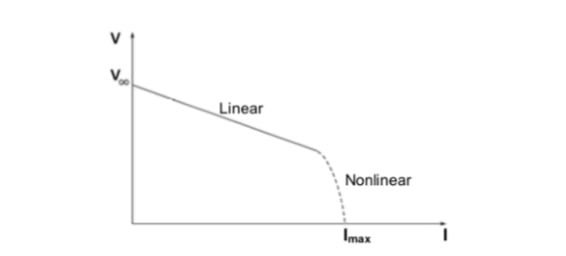
\includegraphics[width=0.65\linewidth]{Figs/terminal_voltage_current_linear.jpg}
  \caption{Terminal voltage vs. current}
  \label{fig:terminal_voltage_vs_current}
\end{figure}

For most cases, many powers sources will exhibit a linear variation of R for small current values, with nonlinear behaviour at higher currents.
The linear part of the curve can be described by:
\[
V = V_{\infty} - RI
\]
where R is the \textit{output resistance of the powers source}.
In this linear regime, according to Thevenin's theorem, the power source is completely represented by the equivalent circuit shown below.

\begin{figure}[htbp]            % h=here, t=top, b=bottom, p=page float
  \centering
  
\includegraphics[width=0.65\linewidth]{Figs/power_source.png}
  \caption{Equivalent circuit of an electric power source.}
  \label{fig:power_source}
\end{figure}


The output resistance (\textit{R}) can be determined by attaching different external resistances of the load ($R_{l}$) to the power source, and measuring the current and voltage with a multimeter.
\ref{fig:two_circuits} shows two possible ways of doing this. Both would be equivalent \textbf{if} the multimeter were ideal.
However, in this exercuse we will measure with real, not ideal, multimeters.

\begin{figure}[htbp]            % h=here, t=top, b=bottom, p=page float
  \centering
  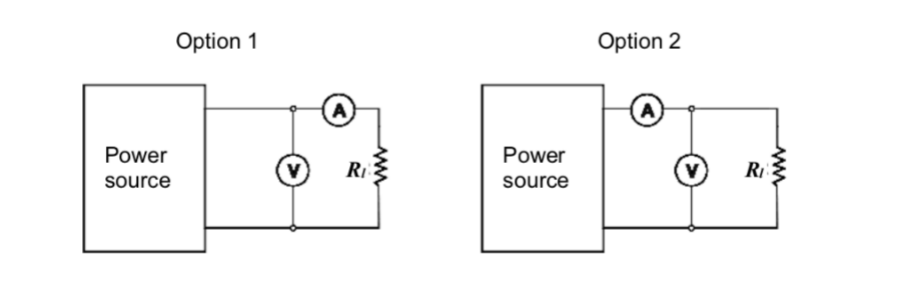
\includegraphics[width=0.65\linewidth]{Figs/two_circuits.png}
  \caption{Possible circuits for determining the output resistance of a power source}
  \label{fig:two_circuits}
\end{figure}

\section{Pre-Lab Exercises}

Without connecting circuits and making measurements, we can expect the the voltmeter and ammeter readings to differ between the two options due to current and voltage leakage.
More specifically, in option 1, we can expect the current to differ as the voltmeter allows some current to pass through. The amount of leakage will depend on the load resistance.
Similarly, in option 2, we can expect that the voltage will differ as the ammeter will draw some voltage. Its leakage will too depend on the load resistance.

To calculate the internal resistances of the voltmeter and the ammeter we can use basic current and voltage division.
For the voltmeter, we can calculate the current that we expect to pass through the ammeter and solve for the voltmeter resistance.

\subsection{Ammeter Internal Resistance Derivation}
Starting from Ohm's law: \( V = I(R_A + R_L) \)
Solve for \( R_A \):
\[
\frac{V}{I} = R_A + R_L \quad\Rightarrow\quad R_A = \frac{V}{I} - R_L
\]

\subsection{Voltmeter Internal Resistance Derivation}
Starting from Ohm's Law: \( V = I\left(\frac{R_V R_L}{R_V + R_L}\right) \)
Solve for \( R_V \):
\[
\frac{V}{I} = \frac{R_V R_L}{R_V + R_L} 
\quad\Rightarrow\quad \frac{V}{I}(R_V + R_L) = R_V R_L 
\quad\Rightarrow\quad \frac{V}{I}R_V + \frac{V}{I}R_L = R_V R_L
\]
\[
\frac{V}{I}R_L = R_V\left(R_L - \frac{V}{I}\right) 
\quad\Rightarrow\quad R_V = \frac{\frac{V}{I}R_L}{R_L - \frac{V}{I}} 
= \frac{V R_L}{I R_L - V}
\]
\section{The Experiment}

We began by measuring the resistance values of the provided resistors. 
For the subsequent circuit experiments, we selected the two highest and two lowest resistance values to represent the load resistance conditions for the voltmeter and ammeter configurations, respectively. 
The measured values with their associated uncertainties are presented below.

\label{table_resistor_values}
\begin{table}[htbp]
\centering
\caption{Resistor Values and Uncertainties}
\begin{tabular}{|c|c|c|c|c|c|c|}
\hline
 & $R_{l1}$ & $R_{l2}$ & $R_{l3}$ & $R_{l4}$ & $R_{l5}$ & $R_{l6}$ \\
\hline
Value ($\Omega$) & 100.32 & 219.91 & 461.3 & 2.6760 k & 26.814 k & 101.57 k \\
\hline
Uncertainty ($\Omega$) & $\pm$0.25 & $\pm$0.49 & $\pm$0.1.42 & $\pm$.0005 k & $\pm$0.006 k & $\pm$0.25 k \\
\hline
\end{tabular}
\end{table}

\newpage
\subsection{Circuit Option 1}
\textbf{INCLUDE DIAGRAM/SKETCH OF CIRCUIT OPTION 1}

\begin{table}[htbp]
\centering
\caption{Circuit 1 Readings \& Results}
\begin{tabular}{|c|c|c|c|c|c|c|c|}
\hline
\makecell{Resistance \\ $R_{li}$ ($\Omega$)} & \makecell{Uncertainty \\ $\Delta R_{li}$ ($\Omega$)} & \makecell{Voltage \\ $V$ (V)} & \makecell{Uncertainty \\ $\Delta V$ (V)} & \makecell{Current \\ $I$ (mA)} & \makecell{Uncertainty \\ $\Delta I$ (mA)} & \makecell{Ammeter Res. \\ $R_A$ ($\Omega$)} & \makecell{Uncertainty \\ $\Delta R_A$ ($\Omega$)} \\
\hline
100.32 & $\pm$0.25 & 6.499 & $\pm$0.005 & 63.67 & $\pm$0.18 & 1.78 & $\pm$0.39 \\
\hline
219.91 & $\pm$0.49 & 6.500 & $\pm$0.005 & 29.315 & $\pm$0.064 & 1.85 & $\pm$0.71 \\
\hline
26.814 k & $\pm$60 & 6.501 & $\pm$0.005 & 0.241 & $\pm$0.051 & 161.10 & $\pm$5708.77 \\
\hline
101.57 k & $\pm$250 & 6.501 & $\pm$0.005 & 0.063 & $\pm$0.005 & 1620.48 & $\pm$8193.92 \\
\hline
\cellcolor{gray!50} & \cellcolor{gray!50} & \cellcolor{gray!50} & \cellcolor{gray!50} & \cellcolor{gray!50} & Average: & 446.3 & $\pm$3475.9 \\
\hline
\end{tabular}
\end{table}

From the experimental data, a linear regression was applied to determine the slope $m_2$ and its associated uncertainty. 
The analysis yielded a slope value of $-0.046 \pm 0.004~\Omega$, where the uncertainty was derived through the standard error propagation for linear fitting parameters (see Appendix \ref{app:c_linear_uncertainties}).

The $\chi^2$ analysis and examination of residuals suggest a potential underestimation of the experimental uncertainties. 
The resistance values $R_V$ used in this fit were calculated from voltage, current, and lead resistance measurements, with their uncertainties propagated according to the method detailed in Appendix \ref{app:b_RV_uncertainty}.
\begin{figure}[htbp]            % h=here, t=top, b=bottom, p=page float
  \centering
  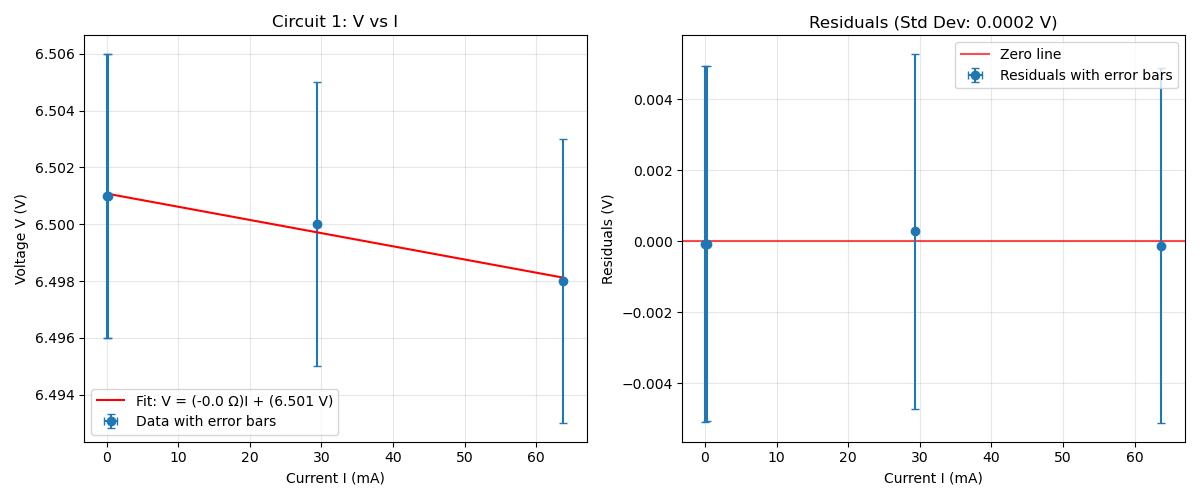
\includegraphics[width=1\linewidth]{Figs/Circuit_1.png}
\caption{Linear regression of voltage versus current measurements for the voltmeter circuit configuration. 
                The slope of $-0.046 \pm 0.004~\Omega$ represents the output resistance of the power source, while the intercept of $6.501 \pm 0.000~V$ corresponds to the open-circuit voltage. 
                The near-zero slope indicates minimal internal resistance in the power supply. 
                The fit quality ($\chi^2 = 0.003$, $\chi^2/\nu = 0.001$, $p = 0.9987$) suggests potential underestimation of measurement uncertainties.
                Reading uncertainity was used for both V and I since they were greater than statistical uncertainties.}    
                \label{fig:circuit_1_fit}
\end{figure}

\newpage

\subsection{Circuit Option 2}
\textbf{INCLUDE DIAGRAM/SKETCH OF CIRCUIT OPTION 2}
\begin{table}[htbp]
\centering
\caption{Circuit 2 Readings \& Results}
\begin{tabular}{|c|c|c|c|c|c|c|c|}
\hline
\makecell{Resistance \\ $R_{li}$ ($\Omega$)} & \makecell{Uncertainty \\ $\Delta R_{li}$ ($\Omega$)} & \makecell{Voltage \\ $V$ (V)} & \makecell{Uncertainty \\ $\Delta V$ (V)} & \makecell{Current \\ $I$ (mA)} & \makecell{Uncertainty \\ $\Delta I$ (mA)} & \makecell{Voltmeter Res. \\ $R_V$ ($\Omega$)} & \makecell{Uncertainty \\ $\Delta R_V$ ($\Omega$)} \\
\hline
100.32 & $\pm$0.25 & 6.386 & $\pm$0.005 & 63.60 & $\pm$0.18 & $-1.13 \times 10^5$ & $\pm$4.94$\times 10^5$ \\
\hline
219.91 & $\pm$0.49 & 6.448 & $\pm$0.005 & 29.322 & $\pm$0.064 & $7.05 \times 10^6$ & $\pm$7.27$\times 10^8$ \\
\hline
26.814 k & $\pm$59 & 6.501 & $\pm$0.005 & 0.243 & $\pm$0.051 & $1.18 \times 10^7$ & $\pm$1.09$\times 10^9$ \\
\hline
101.57 k & $\pm$250 & 6.501 & $\pm$0.005 & 0.065 & $\pm$0.005 & $6.53 \times 10^6$ & $\pm$3.29$\times 10^7$ \\
\hline
\cellcolor{gray!50} & \cellcolor{gray!50} & \cellcolor{gray!50} & \cellcolor{gray!50} & \cellcolor{gray!50} & Average: & $6.31 \times 10^6$ & $\pm$4.62$\times 10^8$ \\
\hline
\end{tabular}
\end{table}

From the experimental data, a linear regression was applied to determine the slope $m_2$ and its associated uncertainty. 
The analysis yielded a slope value of $-1.813 \pm 0.003~\Omega$, where the uncertainty was derived through the standard error propagation for linear fitting parameters (see Appendix \ref{app:c_linear_uncertainties}).

The $\chi^2$ analysis and examination of residuals suggest a potential underestimation of the experimental uncertainties. 
The resistance values $R_A$ used in this fit were calculated from voltage and current measurements, with their uncertainties propagated according to the method detailed in Appendix \ref{app:a_RA_uncertainty}.

\begin{figure}[htbp]
  \centering
  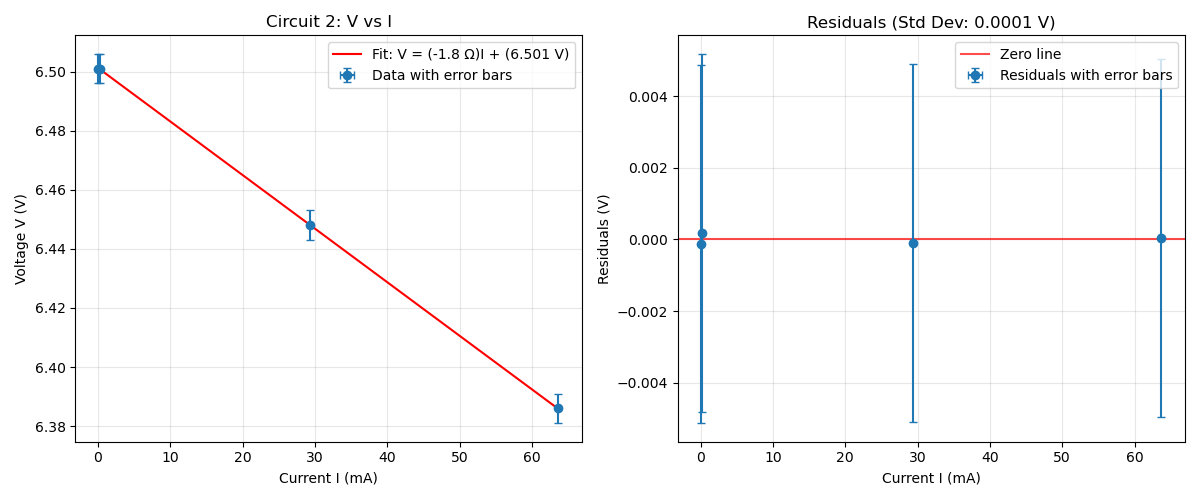
\includegraphics[width=1\linewidth]{Figs/Circuit_2.png}
    \caption{Linear regression of voltage versus current measurements showing an ideal voltage source behavior. 
                The slope of $-1.813 \pm 0.003~\Omega$ represents the effective circuit resistance, while the intercept of $6.501 \pm 0.000~V$ corresponds to the source voltage. 
                The fit quality ($\chi^2 = 0.003$, $\chi^2/\nu = 0.001$, $p = 0.9987$) suggests potential underestimation of measurement uncertainties.
                Reading uncertainity was used for both V and I since they were greater than statistical uncertainties.}
    \label{fig:circuit_2_fit}
\end{figure}

\section{Analysis}

\subsection{Interal Resistance Using R\_V}

The internal resistance of the power source can be derived from the relationship between the measured resistance $m_1$, the voltmeter resistance $R_V$, and the internal resistance $R_{internal}$. 
The measured resistance $m_1$ represents the parallel combination of the voltmeter resistance and the internal resistance:

\begin{align*}
m_1 = \frac{R_V \cdot R_{internal}}{R_V + R_{internal}}
\end{align*}

Solving this equation for $R_{internal}$:

\begin{align*}
m_1 (R_V + R_{internal}) &= R_V \cdot R_{internal} \\
m_1 R_V + m_1 R_{internal} &= R_V \cdot R_{internal} \\
m_1 R_V &= R_V \cdot R_{internal} - m_1 R_{internal} \\
m_1 R_V &= R_{internal} (R_V - m_1)
\end{align*}

Thus, the explicit expression for the internal resistance is:

\begin{align*}
R_{internal} = \frac{m_1 \cdot R_V}{R_V - m_1}
\end{align*}

\subsection{Interal Resistance Using R\_A}

The internal resistance of the power source can also be derived from the relationship between the measured resistance $m_2$, the calculated resistance $R_A$, and the internal resistance $R_{internal}$. 
The measured resistance $m_2$ represents the parallel combination of the resistance $R_A$ and the internal resistance:

\begin{align*}
m_2 = \frac{R_A \cdot R_{internal}}{R_A + R_{internal}}
\end{align*}

Solving this equation for $R_{internal}$:

\begin{align*}
m_2 (R_A + R_{internal}) &= R_A \cdot R_{internal} \\
m_2 R_A + m_2 R_{internal} &= R_A \cdot R_{internal} \\
m_2 R_A &= R_A \cdot R_{internal} - m_2 R_{internal} \\
m_2 R_A &= R_{internal} (R_A - m_2)
\end{align*}

Thus, the explicit expression for the internal resistance is:

\begin{align*}
R_{internal} = \frac{m_2 \cdot R_A}{R_A - m_2}
\end{align*}

\section{Conclusion}

\label{last_page}

\newpage
% \bibliographystyle{iclr2022_conference}
% \bibliography{PHY293_Resistance_Exercise}

\appendix

\section{Uncertainty Derivation for Resistance Measurement R\_A}
\label{app:a_RA_uncertainty}

\subsection*{Step 1: Uncertainty in Division $\frac{V}{I}$}
\begin{align*}
z = \frac{V}{I} \quad \Rightarrow \quad \left(\frac{\sigma_z}{z}\right)^2 &= \left(\frac{\sigma_V}{V}\right)^2 + \left(\frac{\sigma_I}{I}\right)^2 \quad \Rightarrow \quad \sigma_{term1} = \frac{V}{I} \cdot \sqrt{\left(\frac{\sigma_V}{V}\right)^2 + \left(\frac{\sigma_I}{I}\right)^2}
\end{align*}

\subsection*{Step 2: Uncertainty in Subtraction $R_A = term1 - R_{li}$}
\begin{align*}
R_A = A - B \quad \Rightarrow \quad \sigma_{R_A} = \sqrt{\sigma_A^2 + \sigma_B^2} \quad \Rightarrow \quad \sigma_{R_A} = \sqrt{\sigma_{term1}^2 + \sigma_{R_{li}}^2}
\end{align*}

\subsection*{Complete Uncertainty Propagation}
\begin{align*}
\sigma_{R_A} &= \sqrt{\left[\frac{V}{I} \cdot \sqrt{\left(\frac{\sigma_V}{V}\right)^2 + \left(\frac{\sigma_I}{I}\right)^2}\right]^2 + \sigma_{R_{li}}^2} \quad \Rightarrow \quad \sigma_{R_A} = \sqrt{\left(\frac{V}{I}\right)^2 \cdot \left[\left(\frac{\sigma_V}{V}\right)^2 + \left(\frac{\sigma_I}{I}\right)^2\right] + \sigma_{R_{li}}^2}
\end{align*}

Where: $\sigma_V = \texttt{dV}$, $\sigma_I = \texttt{dI}$, $\sigma_{R_{li}} = \texttt{dR\_li}$


\newpage

\section{Uncertainty Derivation for Resistance Measurement R\_V}
\label{app:b_RV_uncertainty}

\subsection*{Step 1: Uncertainty in Numerator $N = V \cdot R_{li}$}
\begin{align*}
N = V \cdot R_{li} \quad \Rightarrow \quad \left(\frac{\sigma_N}{N}\right)^2 = \left(\frac{\sigma_V}{V}\right)^2 + \left(\frac{\sigma_{R_{li}}}{R_{li}}\right)^2 \quad \Rightarrow \quad \sigma_N = N \cdot \sqrt{\left(\frac{\sigma_V}{V}\right)^2 + \left(\frac{\sigma_{R_{li}}}{R_{li}}\right)^2}
\end{align*}

\subsection*{Step 2: Uncertainty in $D_1 = I \cdot R_{li}$}
\begin{align*}
D_1 = I \cdot R_{li} \quad \Rightarrow \quad \left(\frac{\sigma_{D_1}}{D_1}\right)^2 = \left(\frac{\sigma_I}{I}\right)^2 + \left(\frac{\sigma_{R_{li}}}{R_{li}}\right)^2 \quad \Rightarrow \quad \sigma_{D_1} = D_1 \cdot \sqrt{\left(\frac{\sigma_I}{I}\right)^2 + \left(\frac{\sigma_{R_{li}}}{R_{li}}\right)^2}
\end{align*}

\subsection*{Step 3: Uncertainty in Denominator $D = D_1 - V$}
\begin{align*}
D = D_1 - V \quad \Rightarrow \quad \sigma_D = \sqrt{\sigma_{D_1}^2 + \sigma_V^2}
\end{align*}

\subsection*{Step 4: Uncertainty in Quotient $R_V = \frac{N}{D}$}
\begin{align*}
R_V = \frac{N}{D} \quad \Rightarrow \quad \left(\frac{\sigma_{R_V}}{R_V}\right)^2 = \left(\frac{\sigma_N}{N}\right)^2 + \left(\frac{\sigma_D}{D}\right)^2 \quad \Rightarrow \quad \sigma_{R_V} = R_V \cdot \sqrt{\left(\frac{\sigma_N}{N}\right)^2 + \left(\frac{\sigma_D}{D}\right)^2}
\end{align*}

\subsection*{Final Combined Expression}
\begin{align*}
\sigma_{R_V} = \frac{V \cdot R_{li}}{I \cdot R_{li} - V} \cdot \sqrt{\left(\frac{\sigma_V}{V}\right)^2 + \left(\frac{\sigma_{R_{li}}}{R_{li}}\right)^2 + \left(\frac{\sigma_{I \cdot R_{li}}}{I \cdot R_{li}}\right)^2 + \left(\frac{\sigma_V}{I \cdot R_{li} - V}\right)^2}
\end{align*}

Where: $\sigma_V = \texttt{dV}$, $\sigma_I = \texttt{dI}$, $\sigma_{R_{li}} = \texttt{dR\_li}$

\newpage

\section{Linear Regression with Uncertainty Propagation}
\label{app:c_linear_uncertainties}

\subsection*{Linear Model and Definitions}
\begin{align*}
y = mx + b \quad \text{where} \quad N = \text{number of data points}
\end{align*}

\subsection*{Key Quantities}
\begin{align*}
\Delta &= N \sum x_i^2 - \left(\sum x_i\right)^2 \\
S_x &= \sum x_i, \quad S_y = \sum y_i, \quad S_{xx} = \sum x_i^2, \quad S_{xy} = \sum x_i y_i
\end{align*}

\subsection*{Parameter Estimation}
\begin{align*}
m &= \frac{N \cdot S_{xy} - S_x \cdot S_y}{\Delta} \quad \Rightarrow \quad \text{slope} \\
b &= \frac{S_y - m \cdot S_x}{N} \quad \Rightarrow \quad \text{intercept}
\end{align*}

\subsection*{Residuals and Variance}
\begin{align*}
\hat{y}_i &= b + m x_i \quad \Rightarrow \quad \text{predicted values} \\
r_i &= y_i - \hat{y}_i \quad \Rightarrow \quad \text{residuals} \\
\sigma_y^2 &= \sqrt{\frac{\sum r_i^2}{N-2}} \quad \Rightarrow \quad \text{standard error of estimate}
\end{align*}

\subsection*{Parameter Uncertainties}
\begin{align*}
\sigma_m &= \sqrt{\frac{\sigma_y^2 \cdot N}{\Delta}} \quad \Rightarrow \quad \text{slope uncertainty} \\
\sigma_b &= \sqrt{\frac{\sigma_y^2 \cdot S_{xx}}{\Delta}} \quad \Rightarrow \quad \text{intercept uncertainty}
\end{align*}

\subsection*{Chi-Squared Analysis}
\begin{align*}
\chi^2 &= \sum \left(\frac{y_i - \hat{y}_i}{\sigma_{y_i}}\right)^2 \quad \Rightarrow \quad \text{goodness of fit} \\
\chi_\nu^2 &= \frac{\chi^2}{N-2} \quad \Rightarrow \quad \text{reduced chi-squared} \\
p &= 1 - F(\chi^2, N-2) \quad \Rightarrow \quad \text{p-value}
\end{align*}

Where: $\sigma_{y_i}$ are the individual y-uncertainties, $F$ is the chi-squared CDF

\end{document}